\documentclass{article}
\usepackage[utf8]{inputenc}
\usepackage{graphicx}
\usepackage{geometry}
\geometry{a4paper, total={16cm, 24cm}, top=2cm}
\usepackage{amsmath}
\usepackage{amssymb}
\usepackage{blindtext}
\usepackage{hyperref}
\usepackage{wallpaper}
\usepackage{siunitx}
\graphicspath{ {img/} }
\title{\Huge Digital Circuits\\\LARGE Lab Exercise 1}
\author{Steffen Petersen | au722120 \\ Daniel Pihl | au712814}
\date{14. October 2022}
\hypersetup{
    colorlinks=true,
    linkcolor=black,
    filecolor=magenta,      
    urlcolor=cyan,
    pdfpagemode=FullScreen,
}
\setcounter{tocdepth}{4}
\setcounter{secnumdepth}{4}

\begin{document}
\ThisULCornerWallPaper{1}{background1.png}

\begin{titlepage} % Suppresses displaying the page number on the title page and the subsequent page counts as page 1
  \newcommand{\HRule}{\rule{\linewidth}{0.5mm}} % Defines a new command for horizontal lines, change thickness here

    \center % Centre everything on the page
    
    %------------------------------------------------
    %	Headings
    %------------------------------------------------
    \textbf{\space}\\[2cm]   
    \textsc{\LARGE Århus University}\\[1.5cm] % Main heading such as the name of your university/college
    
    \textsc{\Large Computer Technology}\\[0.5cm] % Major heading such as course name
    
    \textsc{\large Project 1}\\[0.5cm] % Minor heading such as course title
    
    %------------------------------------------------
    %	Title
    %------------------------------------------------
    
    \HRule\\[0cm]
    
    {\huge\bfseries Robot Design\\[0.1cm]}
    {\large\bfseries Turtlebot3\\}
    
    \HRule\\[1.5cm]
    
    %------------------------------------------------
    %	Author(s)
    %------------------------------------------------
    
    \begin{minipage}{0.4\textwidth}
      \begin{flushleft}
        \large
        \textit{Authors}\\
        Steffen T. Petersen | AU722120\\
        Daniel Pihl | AU712814
      \end{flushleft}
    \end{minipage}
    \begin{minipage}{0.4\textwidth}
      \begin{flushright}
        \large\vspace{-4mm}
        \textit{Instructors}\\
        Jalil Boudjadar\\
        Mirgita Frasheri
      \end{flushright}
    \end{minipage}
    
    % If you don't want a supervisor, uncomment the two lines below and comment the code above
    %{\large\textit{Author}}\\
    %John \textsc{Smith} % Your name
    
    %------------------------------------------------
    %	Date
    %------------------------------------------------
    
    \vfill\vfill\vfill % Position the date 3/4 down the remaining page
    
    {\large October 28th, 2022} % Date, change the \today to a set date if you want to be precise
    
    %------------------------------------------------
    %	Logo
    %------------------------------------------------
    
    %\vfill\vfill
    %\includegraphics[width=0.2\textwidth]{placeholder.jpg}\\[1cm] % Include a department/university logo - this will require the graphicx package
     
    %----------------------------------------------------------------------------------------
    
    \vfill % Push the date up 1/4 of the remaining page
    
  \end{titlepage}

%\maketitle
%\includegraphics[width=\linewidth, keepaspectratio=true]{tempFront}

\pagebreak

\section*{Abstract}
\addcontentsline{toc}{section}{Abstract}
%In this lab exercise we are to observe the behavior of 6 types of logic gates in their IC versions, where we create simple circuits to test their functions and compare that to our thesis.
In this lab exercise we are to practice logic minimization of digital circuits. We will be briefly covering the theory behind
a few concepts in boolean algebra which are used as tools to simplify and minimize digital circuits.\\
We will also conduct an experiment to verify our expectations based on the theoritcal results.

\vspace{11cm}
\tableofcontents
\pagebreak
%\section*{Main body}
\addcontentsline{toc}{section}{Theory} \addtocounter{section}{1}
\section*{Theory}
\subsection*{Boolean Algebra}\addcontentsline{toc}{subsection}{Boolean Algebra}
Boolean algebra has 3 main rules or operators that are all over. These are the AND, OR and NOT operators, 
where the AND operator is a multiplication sign "$\cdot$", the or is a plus sign "$+$" and the NOT operator usually 
is shown as an overline "$\si{\overline{A}}$" or an apostrophe.\\

\noindent The AND operator is also often not shown, but rather implied, for example if you have two variables, A and B, and you AND these,
you may also just write "AB" instead of "A$\cdot$B".
In practice, the logic operation of an AND is when a series of inputs that are "\textit{ANDed}" together, all have to be a 
logic value 1 for the output to also be logic 1.\\

\noindent The logic operator OR will instead only need 1 of the "\textit{OR'd}" input variables, to be logic 1, in order to output logic 1.\\

\noindent The NOT operation simply inverses the values of whatever it is "\textit{NOT'ing}", for example it could not an entire AND operation,
making it a NAND which will only output logic 0, when all inputs are logic 1.

\subsection*{Karnaugh Maps}\addcontentsline{toc}{subsection}{Karnaugh Maps}
Karnaugh maps or K-maps, is a way to simplify boolean expressions which are too tedious for Boolean algebra. The reduction could be
done with Boolean algebra. However, with the Karnaugh map it is faster and easier.
When constructed the Karnaugh map is used to find the simplest possible forms for the information in the truth table.
Looking at it, adjacent 1's and 0's represent an opportunity to simplify the given expression. The minterms for the final expression
are found by circling groups of 1's or 0's on the map. Circles must be rectangular and must have an area that is a power of two. When doing
the circles one should always aim to make the largest possible rectangle of either 1's or 0's. The circles are allowed to overlap to ensure
all of ones chosen values are being used. \\[0.05cm]

\noindent Typically it's done using groups of 1's, because this would be simplified into an expression Y, which directly equals the given expression.
However, if it's easier to group the 0's, the simplification of that expression, is $\overline{Y}$. This means you would need to
invert it, to get a final result, Y.\\[0.05cm]

\noindent Karnaugh maps can also have a "don't care" condition. This condition specifies some minterms, or rather, slots in the KMap, that represent
an input about which, the desired function of the expression doesn't rely. This means, that for the sake of making the simplification even better,
you can choose what these slots will be in the KMap, they can function as either 1's or 0's.\\
Usually these are represented by an "X" in the KMap instead of a 0 or 1.\\[0.05cm]

\noindent Here is an example of a general setup of a 4-variable Karnaugh Map (See \hyperlink{kmapsample}{Figure 1})
\begin{figure}[h]
    \centering
    \caption{4-Variable Karnaugh Map}\label{fig:kmapsample}\hypertarget{kmapsample}{\space}
    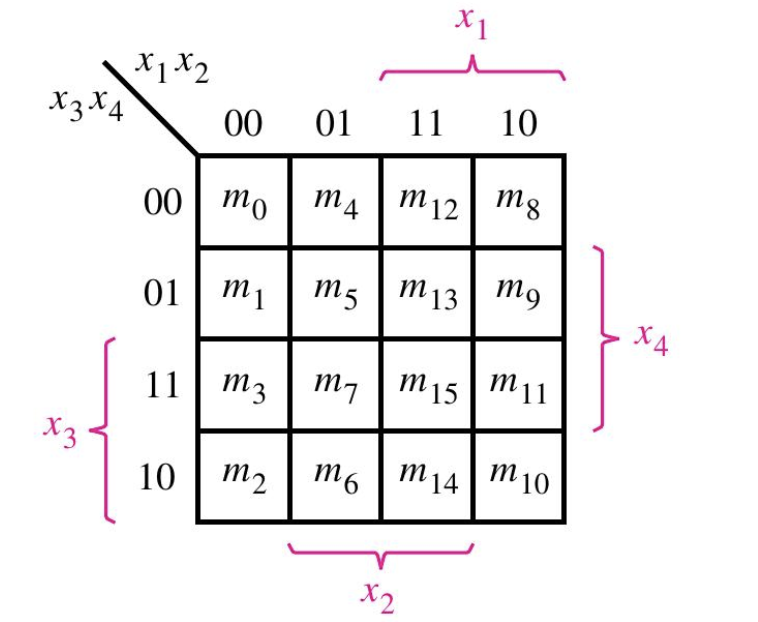
\includegraphics[width=0.42\linewidth, keepaspectratio=true]{kmapSample}
\end{figure}

\pagebreak

\addcontentsline{toc}{section}{Exercise 1} \addtocounter{section}{1}
\section*{Exercise 1}
\noindent In the following three subtasks we are to simplify the given expressions using boolean algebra.
\subsubsection*{a.} \addcontentsline{toc}{subsection}{a.}
\[Y1= A\bar{B} + A(\overline{B+C}) + B(\overline{B+C})\]
Applying DeMorgan Theorem we get:
\[Y1 = A\bar{B} + A\bar{B}\bar{C} + B\bar{B}\bar{C}\]
Applying Complement law: 
\[Y1 = A\bar{B} + A\bar{B}\bar{C}\]
Applying the Absorption law we get the final simplified expression:
\[Y1 = A\bar{B}\]

\subsubsection*{b.} \addcontentsline{toc}{subsection}{b.}
\[Y2 =  BC + A\bar{B}\bar{C} + \bar{A}\bar{B}\bar{C} + A\bar{B}C + ABC\]
Applying Complementary law on $A\bar{B}C$ and $ABC$: 
\[Y2 = BC + A\bar{B}\bar{C} + \bar{A}\bar{B}\bar{C} + AC\]
Applying Complementary law on $A\bar{B}\bar{C}$ and $\bar{A}\bar{B}\bar{C}$:
\[Y2 = BC + \bar{B}\bar{C} + AC\]


\subsubsection*{c.} \addcontentsline{toc}{subsection}{c.}
\[Y3 =  (A\bar{B}(C+BD) + \bar{A}\bar{B})C \]
Applying Distributive law: 
\[Y3 = \bar{B}C(A(C+BD)+\bar{A})\]
Applying Absorption law: 
\[Y3 = \bar{B}C(C+BD+\bar{A})\]
Distributing: 
\[Y3 = \bar{B}C + B\bar{B}CD + \bar{A}\bar{B}C\]
Since the following is true: \\
\[B\bar{B} = 0\]
\[A + 0 = A\]
we get: 
\[Y3 = \bar{B}C + \bar{A}\bar{B}C\]
According to the dominance law, we get the final simplified expression: 
\[Y3 = \bar{B}C\]\\[0.5cm]

\addcontentsline{toc}{section}{Exercise 2} \addtocounter{section}{1}
\section*{Exercise 2}
In this exercise we are to use a Karnaugh map to simplify the folowing expression:
\[Y4 = \bar{A}\bar{B}\bar{C}\bar{D} + \bar{A}\bar{B}C\bar{D} + \bar{A}BC\bar{D} + A\bar{B}\bar{C}\bar{D} + ABCD + A\bar{B}CD\]

\noindent In order to construct our KMap we need to find our minterms for the Y4 expression, where we look at which binary 
combinations, will produce an output of logic 1. \\
These binary combinations are converted to decimal numbers, for our easier understanding, and then written up as 
the following minterm:
\[\sum m (0, 2, 4, 6, 8, 11, 15)\]
With this minterm for our expression, we can construct the following KMap:
\begin{figure}[h]
  \centering
  \caption{KMap of Y4}\label{fig:Y4}\hypertarget{Y4}{\space}
  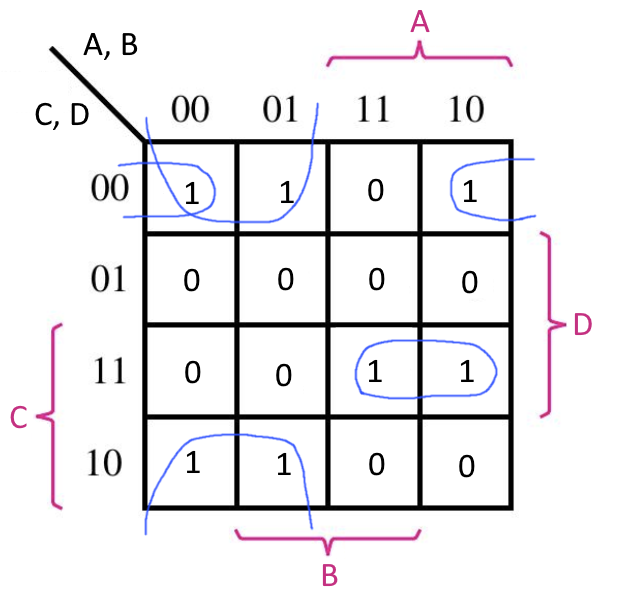
\includegraphics[width=0.4\linewidth, keepaspectratio=true]{Y4KMAP}
\end{figure}\\
\noindent These groups of 1's will amount to the following simplified expression:
\[Y4 = ACD + \bar{B}\bar{C}\bar{D} + \bar{A}\bar{D}\]

\pagebreak

\addcontentsline{toc}{section}{Exercise 3} \addtocounter{section}{1}
\section*{Exercise 3}
\subsubsection*{a.} \addcontentsline{toc}{subsection}{a.} %\addtocounter{subsection}{1}
Here is our circuit in PSpice: 
\begin{figure}[h]
  \centering
  \caption{PSpice circuit}\label{fig:PSpice}\hypertarget{PSpice}{\space}
  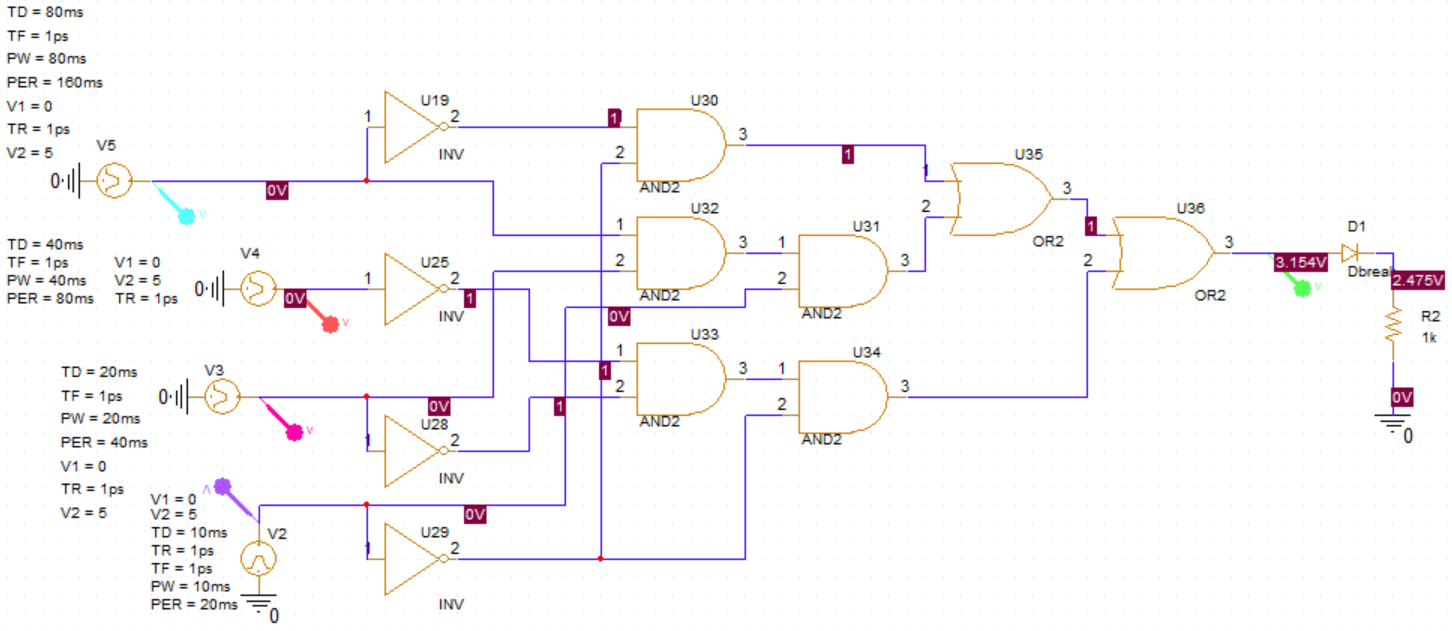
\includegraphics[width=0.85\linewidth, keepaspectratio=true]{SimulationCircuit}
\end{figure}

\noindent After constructing the circuit we tried to simulate it in PSpice to see if our results would match with our theoretical results. We got the following: \\
\begin{figure}[h]
  \centering
  \caption{PSpice simulation}\label{fig:PSpice}\hypertarget{PSpice}{\space}
  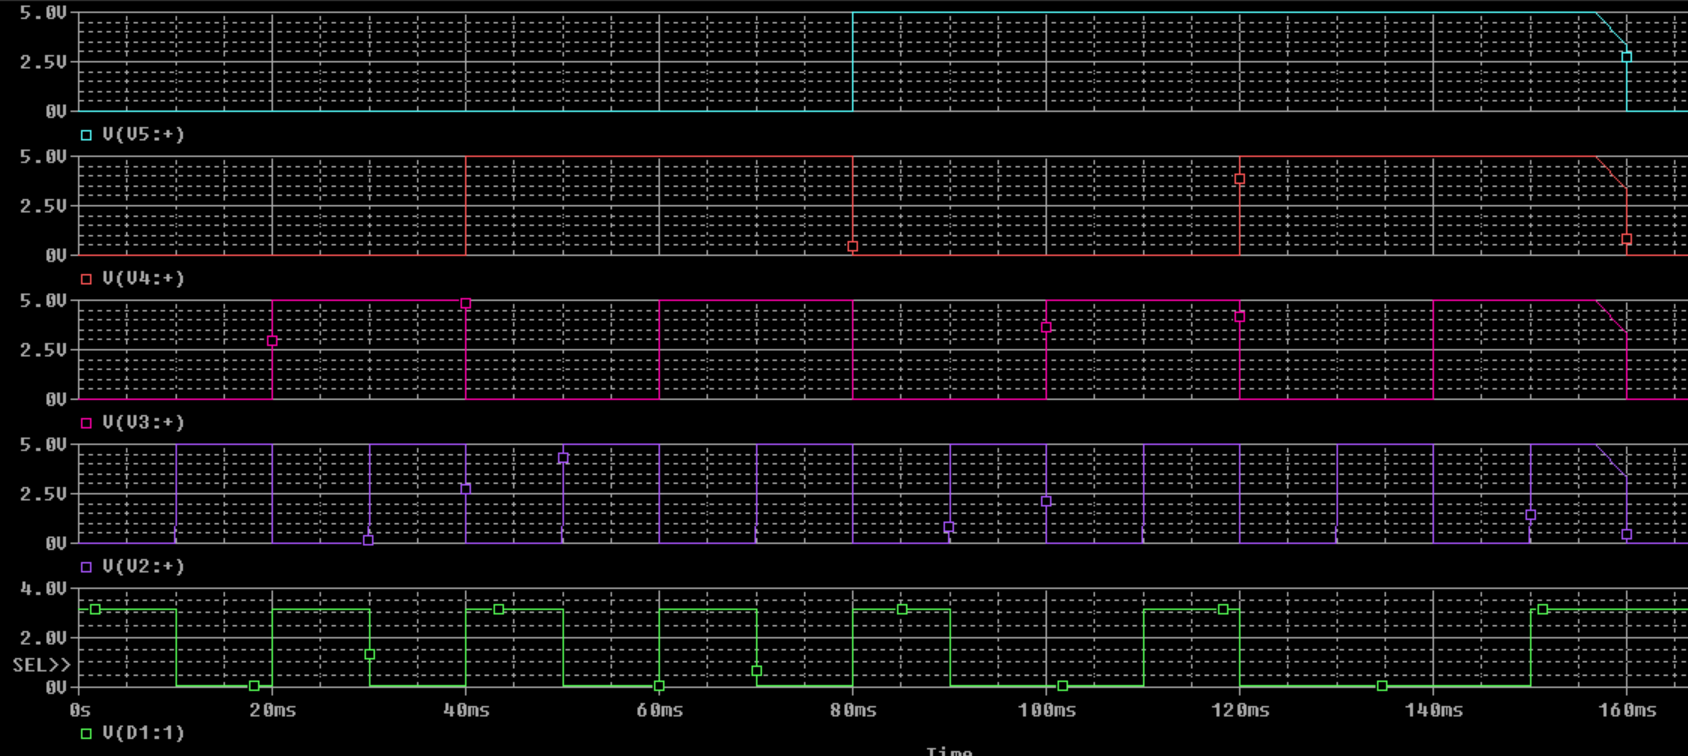
\includegraphics[width=0.85\linewidth, keepaspectratio=true]{SimulationResult}
\end{figure}

\noindent Deducting the simulation, we can see it outputs the expected theoretcial result.


\pagebreak
\subsubsection*{b.} \addcontentsline{toc}{subsection}{b.}
Our picture of the breadboard construction. The four "loose" wires here, each represent an input (A, B, C, D) and the wire to the right is the output.


%\addcontentsline{toc}{subsection}{Testing and Results} \addtocounter{subsection}{1}
%\subsection*{Testing and Results}

\begin{figure}[h] 
  \centering
  \caption{Our setup}\label{fig:setup}\hypertarget{setup}{\space}
  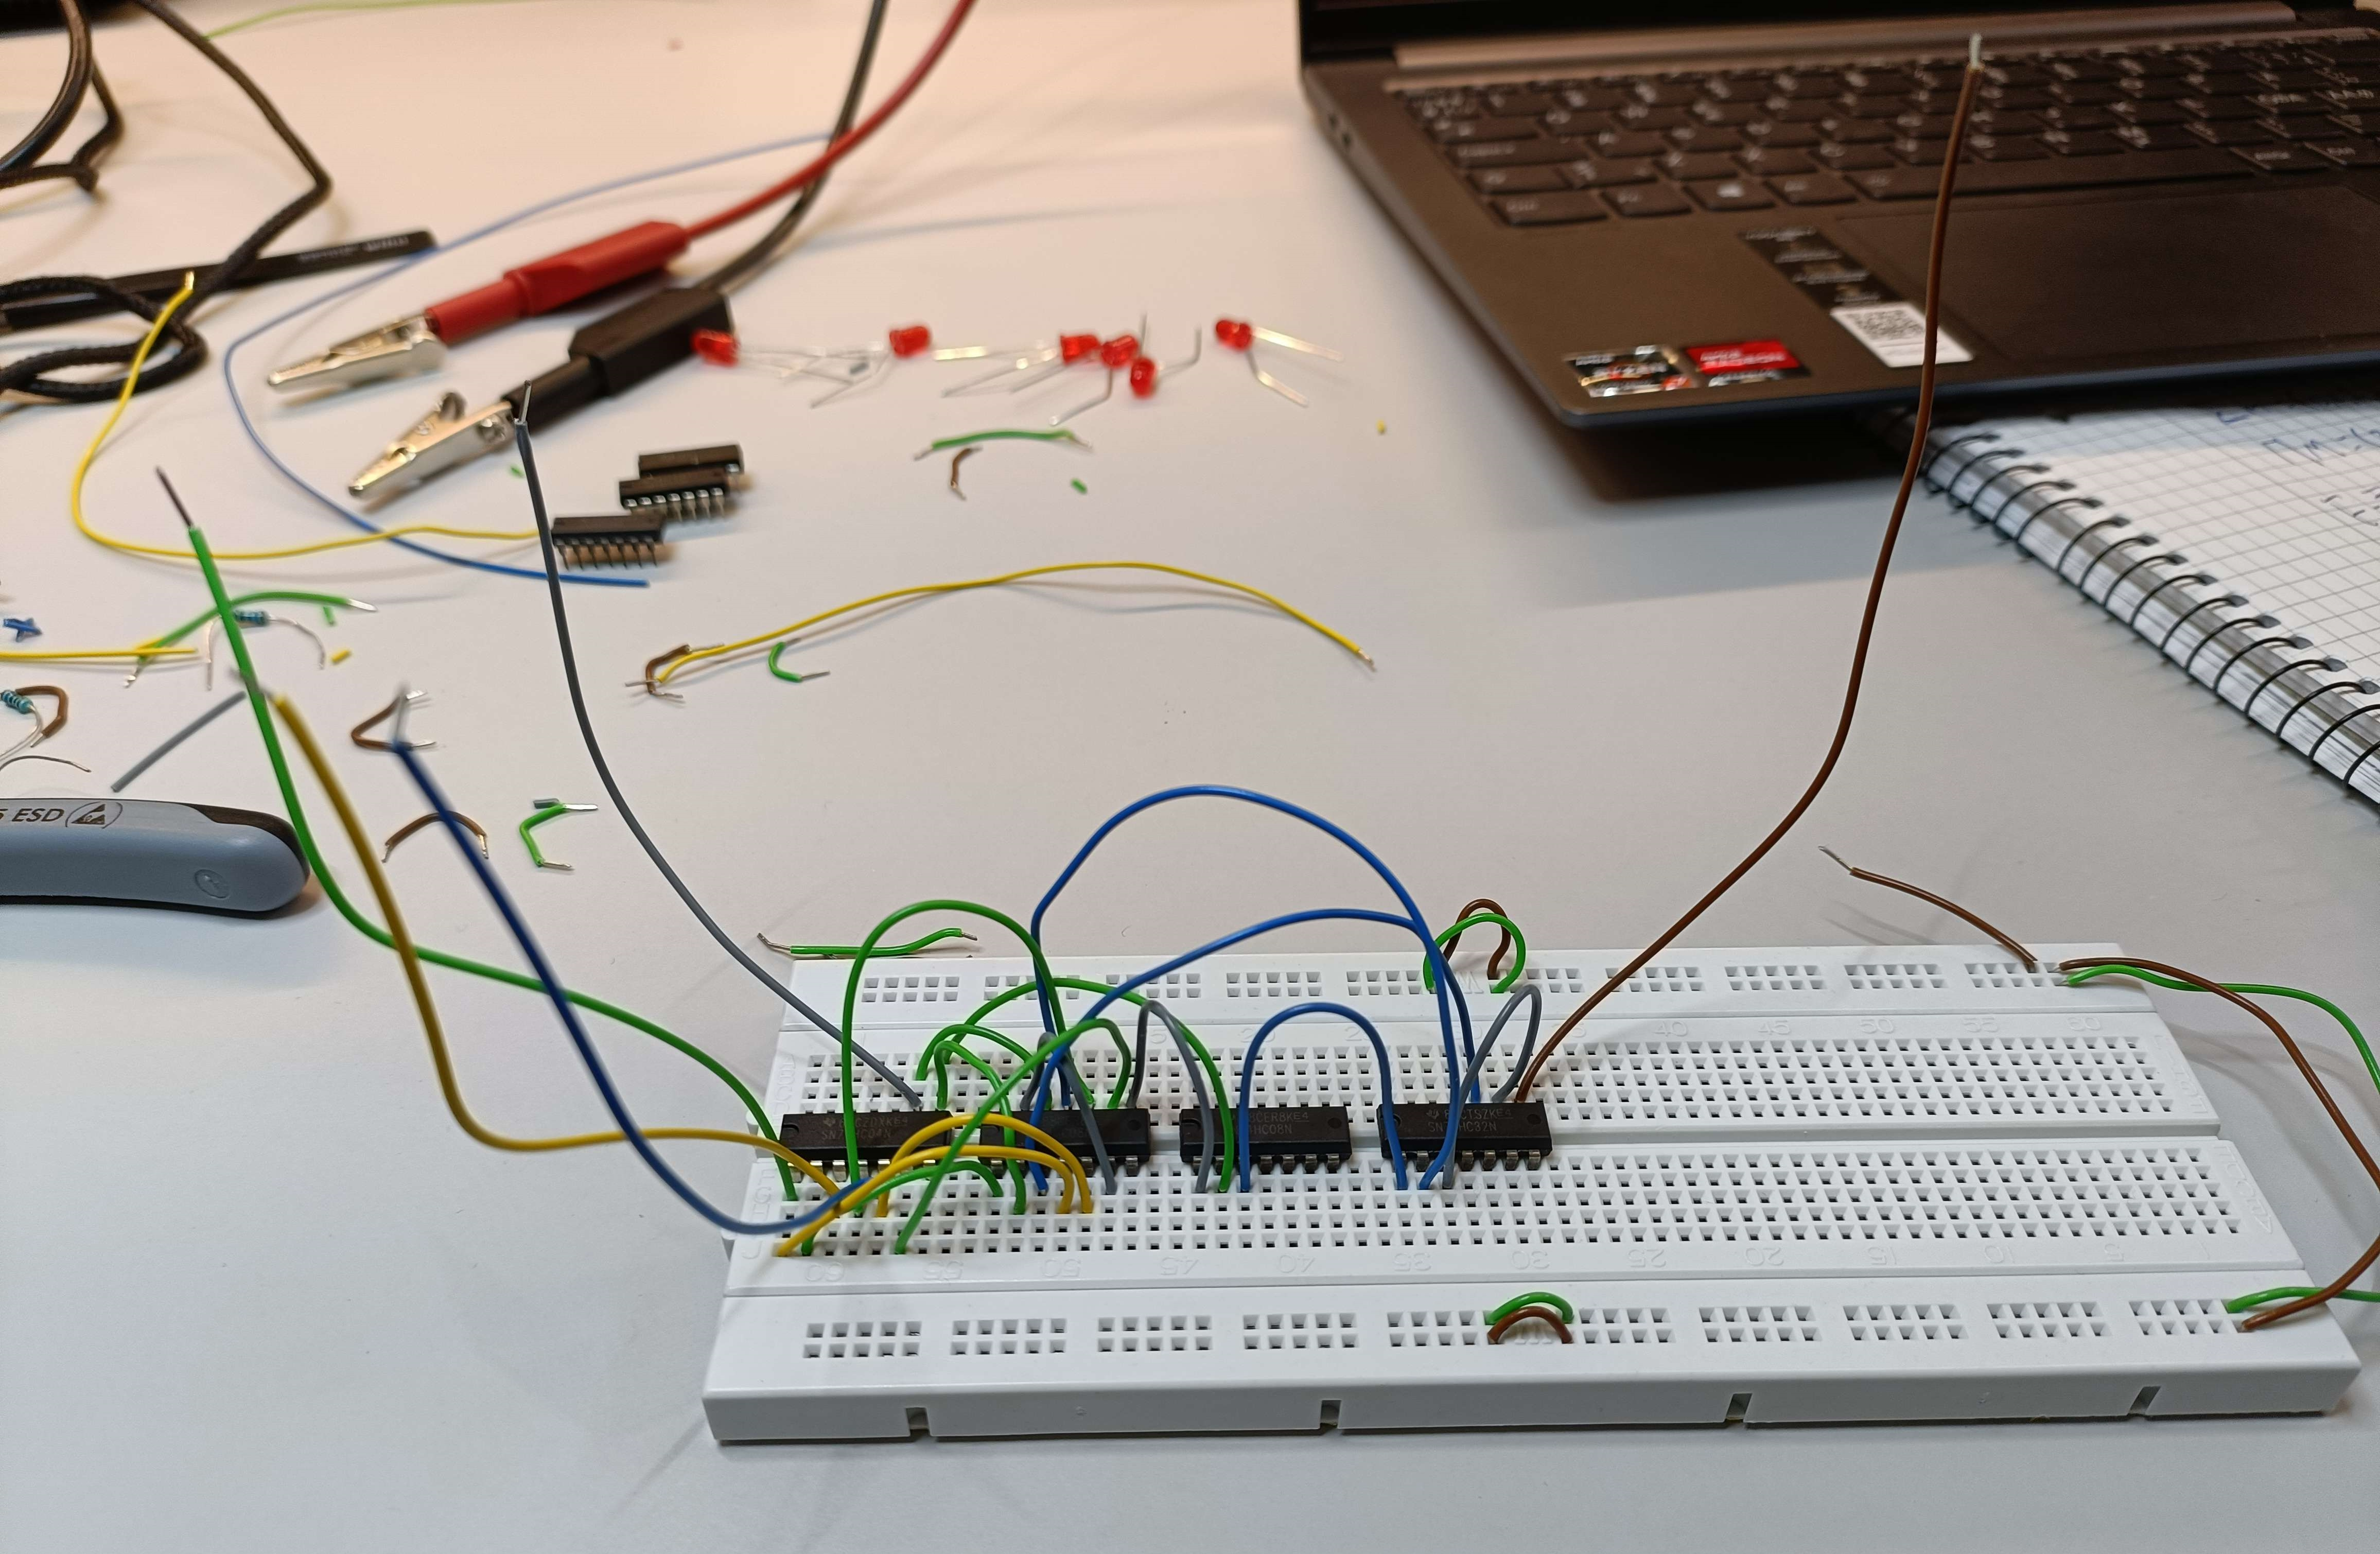
\includegraphics[width=0.8\linewidth, keepaspectratio=true]{exercise3setup}
\end{figure}
% \includegraphics[width=0.92\linewidth, keepaspectratio=true]{maintask}
% \section*{Opgave 2.12 | I-bogen}
%\includegraphics[width=\linewidth, keepaspectratio=true]{maintask}
%{\centering \includegraphics[keepaspectratio=true]{task1}\\}

\subsubsection*{c.} \addcontentsline{toc}{subsection}{c.}
Comparing our experimental results with the theoretical and simulated ones, we of course expected them to match up. 
Lo and behold they did, and below in our truthtable \hyperlink{Y4Table}{(see table 1)}, this can be seen, when comparing
it to our simulation results (see \hyperlink{PSpice}{PSpice results}), where each period is 10ms ending at 160ms. 

% AND & NAND gates
\begin{table}[h]
    \begin{center}
    \caption{Y4 Truth table}\label{tab:table1}\hypertarget{Y4Table}{\space}
    \vspace{3pt}
    \begin{tabular}{|c|c|c|c||c|c|}
      \hline A & B & C & D & Expected out & Actual out\\
      \hline \hline 0 & 0 & 0 & 0 & 1 & 1\\
      \hline 0 & 0 & 0 & 1 & 0 & 0\\
      \hline 0 & 0 & 1 & 0 & 1 & 1\\
      \hline 0 & 0 & 1 & 1 & 0 & 0\\
      \hline 0 & 1 & 0 & 0 & 1 & 1\\
      \hline 0 & 1 & 0 & 1 & 0 & 0\\
      \hline 0 & 1 & 1 & 0 & 1 & 1\\
      \hline 0 & 1 & 1 & 1 & 0 & 0\\
      \hline 1 & 0 & 0 & 0 & 1 & 1\\
      \hline 1 & 0 & 0 & 1 & 0 & 0\\
      \hline 1 & 0 & 1 & 0 & 0 & 0\\
      \hline 1 & 0 & 1 & 1 & 1 & 1\\
      \hline 1 & 1 & 0 & 0 & 0 & 0\\
      \hline 1 & 1 & 0 & 1 & 0 & 0\\
      \hline 1 & 1 & 1 & 0 & 0 & 0\\
      \hline 1 & 1 & 1 & 1 & 1 & 1\\
      \hline
  \end{tabular}
\end{center}
\end{table}

\pagebreak


\section*{Conclusion}

\addcontentsline{toc}{section}{Conclusion} \addtocounter{section}{1}
All in all the lab exercise was a success, given the real world experiment matched up with our theory and expectations.

\vspace{3mm}




\end{document}